%%%%%%%%%%%%%%%%%%%%%%%%%%%%%%%%%%%%%%%%%
% Programming/Coding Assignment
% LaTeX Template
%
% This template has been downloaded from:
% http://www.latextemplates.com
%
% Original author:
% Ted Pavlic (http://www.tedpavlic.com)
%
% Note:
% The \lipsum[#] commands throughout this template generate dummy text
% to fill the template out. These commands should all be removed when
% writing assignment content.
%
% This template uses a Perl script as an example snippet of code, most other
% languages are also usable. Configure them in the "CODE INCLUSION
% CONFIGURATION" section.
%
%%%%%%%%%%%%%%%%%%%%%%%%%%%%%%%%%%%%%%%%%

%----------------------------------------------------------------------------------------
% PACKAGES AND OTHER DOCUMENT CONFIGURATIONS
%----------------------------------------------------------------------------------------

\documentclass{scrartcl}

\usepackage[T1]{fontenc}
\usepackage[utf8x]{inputenc}

\usepackage{fancyhdr} % Required for custom headers
\usepackage{lastpage} % Required to determine the last page for the footer
\usepackage{extramarks} % Required for headers and footers
\usepackage[usenames,dvipsnames]{color} % Required for custom colors
\usepackage{graphicx} % Required to insert images
\usepackage{listings} % Required for insertion of code
\usepackage{courier} % Required for the courier font

\usepackage{hyperref}

\linespread{1.1} % Line spacing

% Set up the header and footer
\pagestyle{fancy}
\lhead{\hmwkAuthorName \\} % Top left header
\chead{\hmwkClass: \hmwkTitle} % Top center head
\rhead{\firstxmark} % Top right header
\lfoot{\lastxmark} % Bottom left footer
\cfoot{} % Bottom center footer
\rfoot{Page\ \thepage\ of\ \protect\pageref{LastPage}} % Bottom right footer
\renewcommand\headrulewidth{0.4pt} % Size of the header rule
\renewcommand\footrulewidth{0.4pt} % Size of the footer rule

\setlength\parindent{0pt} % Removes all indentation from paragraphs

%----------------------------------------------------------------------------------------
%	CODE LISTINGS SETUP
%----------------------------------------------------------------------------------------
\usepackage{color}
\usepackage[usenames,dvipsnames,svgnames,table]{xcolor}
\colorlet{MAROON}{Maroon}
\usepackage{minted}
\providecommand*{\listingautorefname}{Listing}

%----------------------------------------------------------------------------------------
% NAME AND CLASS SECTION
%----------------------------------------------------------------------------------------

\newcommand{\hmwkTitle}{Project 1 -- Using Minimax with Alpha-Beta pruning to play Quarto} % Assignment title
\newcommand{\hmwkDueDate}{Wednesday,\ September\ 18,\ 2013} % Due date
\newcommand{\hmwkClass}{IT3105} % Course/class
\newcommand{\hmwkClassTime}{} % Class/lecture time
\newcommand{\hmwkClassInstructor}{Lecturer: Keith Downing} % Teacher/lecturer
\newcommand{\hmwkAuthorName}{Pablo Liste Garcia \& Dominik Horb} % Your name

%----------------------------------------------------------------------------------------
% TITLE PAGE
%----------------------------------------------------------------------------------------

\title{
\vspace{2in}
\textmd{\textbf{\hmwkClass:\ \hmwkTitle}}\\
\normalsize\vspace{0.1in}\small{Due\ on\ \hmwkDueDate}\\
\vspace{0.1in}\large{\textit{\hmwkClassInstructor\ \hmwkClassTime}}
\vspace{3in}
}

\author{\textbf{\hmwkAuthorName}}
\date{} % Insert date here if you want it to appear below your name

%----------------------------------------------------------------------------------------

\begin{document}

\maketitle

%----------------------------------------------------------------------------------------
% TABLE OF CONTENTS
%----------------------------------------------------------------------------------------

%\setcounter{tocdepth}{1} % Uncomment this line if you don't want subsections listed in the ToC

\newpage
\tableofcontents
\newpage

\section{General Setup}

The first decision our team made after we initially heard of the assignment task,was to use Java as our programming language. This decision was made mainly out of familiarity with the language and because we couldn't find any caveats that would complicate fulfilling the assignment.

We also chose to share our code through a Git repository, which you can access through:

\begin{itemize}
\item \url{https://github.com/dom2503/Quarto}
\end{itemize}

We also wanted to start out with a basic command line interface as it was shown during the lecture and create a graphical interface maybe later on, if there would be time left.

You can see an example of the interface we created in \autoref{fig:basic-interface}.

 \begin{figure}[bth]
 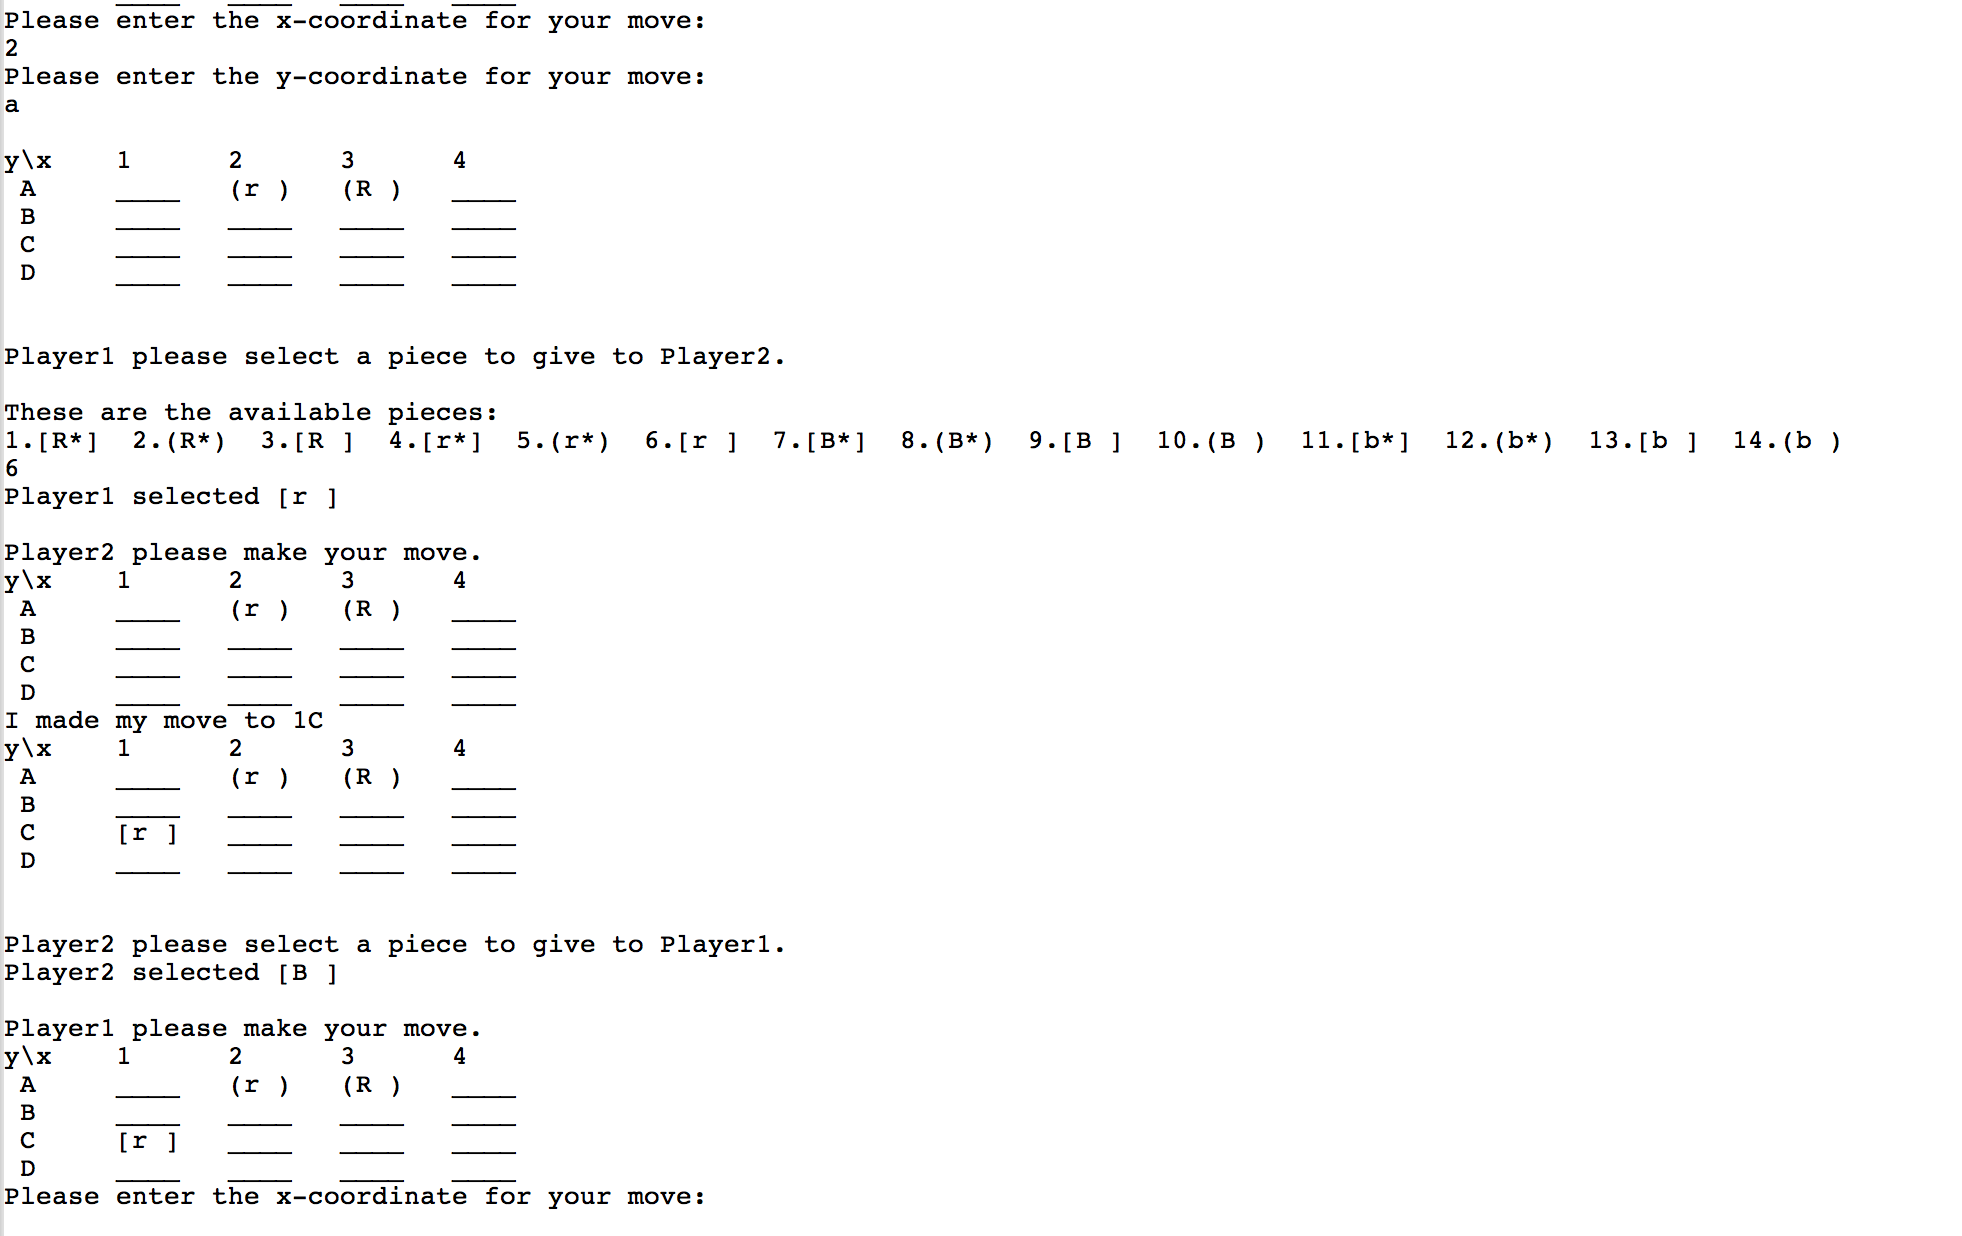
\includegraphics[width=1.0\linewidth]{graphics/basic-interface.png}
\caption{Basic interface of our Quarto game.}\label{fig:basic-interface}
 \end{figure}

The general structure of our code is pretty simple. The main class of the application is \textit{QuartoGame}, which contains the game loop and almost all setup and command line interface parts. The actual game is put together through the \textit{Board} and \textit{Piece} classes and some additional enums for the properties of the pieces.

All the local players that we were supposed to write just needed to be able to pick a next piece and to make a move with the piece that was given to them, as can be seen in the shortened version of our \textit{Player} interface below.

\begin{listing}[H]
\caption{Player interface}
\begin{minted}[linenos=true]{java}
public interface Player {
  public String makeMove();
  public Piece selectPieceForOpponent();
  public void setGivenPiece(Piece givenPiece);
}
\end{minted}
\end{listing}

\section{Evaluation Function}

We first started out thinking about the actual evaluation function for the states of the Quarto game, after we finished the main game logic, the random and the human player. As the main focus was to get the Minimax algorithm working, we wrote a very basic dummy version that just returned a random double value in the beginning.

\begin{listing}[H]
\caption{Dummy evaluation function}
\begin{minted}[linenos=true]{java}
public double evaluateBoard(Board board){
  return rand.nextDouble();
}
\end{minted}
\end{listing}

In the real version later on it should evaluate, whether the current state of the board is good for the player that is supposed to make the next move. A positive value meaning that this is the case and a negative one meaning that the opponent has an advantage.

The state of the game as we look at it at this point, is just the board and the pieces that were already placed.

After our implementation of Minimax had developed into a more mature state we added the two distinctive finishing states of the Quarto game: a draw and the win of the player that set the last piece. As you can see below, we were returning negative infinity for a win, because it is the worst outcome that can be reached and 0.0 for a draw, because no player has an advantage there.

\begin{listing}[H]
\caption{Very basic evaluation function}
\begin{minted}[linenos=true]{java}
public double evaluateBoard(Board board){
    double result;
    if(board.gameWasWon()){
      result = Double.NEGATIVE_INFINITY;
    } else if(board.isDraw()){
      result = 0.0;
    } else {
      result = rand.nextDouble();
    }

    return result;
}
\end{minted}
\end{listing}

Figuring out the next evolutionary step of the evaluation process proofed to be a bit more difficult though. What we somehow concluded was, that leaving a lot of nearly completed rows, that contained three pieces with one or two identical properties for the next player is somehow a bad decision.

Playing in a way that the other player doesn't have a choice but to leave open nearly finished lines however -- preferably with only pieces left that would finish these -- would be good decision making.

We therfore replaced the random value in the else block with the following code that simply counts the number of lines that fulfill these criterias:

\begin{listing}[H]
\caption{Counting nearly finished lines.}
\begin{minted}[linenos=true]{java}
int nearlyFinishedLines = this.getNearlyFinishedLineCount(board);

// the value of 10.0 is arbitrary, it's just to denote that it's good 
// that we don't leave nearly finished lines
if(nearlyFinishedLines == 0){
  return 10.0;
}
// nearly finished lines are bad, because, the next user could maybe finish them 
// with the right piece
return -1.0 * nearlyFinishedLines;
\end{minted}
\end{listing}

After a while we noticed, that even though Minimax was winning against the random player, it was having trouble against the novice. What we figured was, that the heuristic we had was probably not perfect, but should still win against this player.

By talking to the other group we got some hints to help us fix these problems.

The first point was, that we were running minimax two times, both for the selection of the move and the piece. Additionally the piece selection seemed to be somehow faulty then. It was selecting very unintelligently sometimes. While trying to figure out this bug, one member of the other teams we talked to mentioned that we didn't even need to evaluate twice, but that we could simply the piece that we found during the selection of the move -- which  is totally logical, because nothing changes in between.

The second problem we had was that we forgot to multiply the result of the evaluation by -1 when minimizing.

\section{Novice vs. Random}

\begin{tabular}{l c c c}
Runs & Novice & Random & Draws \\
\hline
20 & 20 & 0 & 0  \\
\end{tabular}

\section{Novice vs. Minimax-3}

\begin{tabular}{l c c c}
Runs & Novice & Minimax-3 & Draws \\
\hline
20 & 1 & 19 & 0  \\
\end{tabular}

\section{Minimax-3 vs. Minimax-4}

\begin{tabular}{l c c c}
Runs & Minimax-3 & Minimax-4 & Draws \\
\hline
20 & 3 & 10 & 7  \\
\end{tabular}

\section{Tournament experiences}

\begin{tabular}{l c c c}
Runs & Our Minimax & Marc \& Valerio & Draws \\
\hline
20 & 16 & 3 & 1  \\
\end{tabular}

\begin{tabular}{l c c c}
Runs & Our Minimax & Jan \& Tomas & Draws \\
\hline
20 & 0 & 18 & 2  \\
\end{tabular}

Together with the other groups we decided to use a client-server approach for making the tournament happen. As our software architecture was really well suited for being the server, we inherited the responsibility of implementing this part and figure out the main protocol.

For the implementation we just needed to extend the above mentioned Player interface a bit, so that it also could be used to send some additional messages and implement it in a \textit{RemotePlayer} class: 

\begin{listing}[H]
\caption{Remote player interface}
\begin{minted}[linenos=true]{java}
public interface IRemotePlayer extends Player {
  public void sendMove(int x, int y);
  public void sendMessage(String message);
  public String receiveMessage();
  public void close();
}
\end{minted}
\end{listing}

The only change to our game loop was then to check if the nextPlayer is a remote player, so that we would need to send some information about the made move:

\begin{listing}[H]
\caption{Sending move information.}
\begin{minted}[linenos=true]{java}
Point move = this.currentPlayer.makeMove();
if(this.nextPlayer instanceof IRemotePlayer){
  IRemotePlayer remote = (IRemotePlayer) this.nextPlayer;
  remote.sendMove(move.x, move.y);
}
\end{minted}
\end{listing}

All the other methods of the normal interface could basically be used, just instead of calculating the correct move within \textit{makeMove} for example we just needed to read from the port that was opened on the creation of the object. This setup could also easily be used with two remote players, because every object uses a different port to communicate.

The major problem was then just to get everyone together in order to conduct the real tournament and fix the unavoidable small bugs, the server was just written with a very small dummy client after all.

With one of the groups we wanted to conduct the tournament with, this was working pretty well. We just met with them, discussed the protocol and handed them the .jar file which they could use to test their own client implementation. They just found one bug, which was easily fixable and after this it was working fine, when both implementations where executed on the same machine. 

We also tried to run the tournament over the eduroam network with them, but this was leading to exceptions, for which our best guess is, that it has something to do with linefeed problems between Windows and OS X.

During the games we played against them, we found out, that the heuristic we implemented apparently wasn't really good. They were simply wiping the floor with our Minimax-4 player.

By the time of writing of this report -- three hours before the deadline -- the 2nd team we wanted to battle against sadly hadn't finished their client implementation. We are still hoping, that we will be able to present at least the results table here, but wanted to finish the report now.

\end{document}
